%%%%%%%%%%%%%%%%%%%%%%%%%%%%%%%%%%%%%%%%%%%%%%%%%%%%%%%%%%%%%%%%%%%%%%%%%%%%%%%%%%%%%%%
%%%%%%%%%%%%%%%%%%%%%%%%%%%%%%%%%%%%%%%%%%%%%%%%%%%%%%%%%%%%%%%%%%%%%%%%%%%%%%%%%%%%%%%
%%%%%%%%%%%%%%%%%%%%%%%%%%%%%%%%%%%%%%%%%%%%%%%%%%%%%%%%%%%%%%%%%%%%%%%%%%%%%%%%%%%%%%%
\section{Minimização de $||h(x)-a||^2$} 



\index{Minimização, métodos!Método de Newton}
%\index{Problema inverso!Não linear}
\index{Minimização do erro quadrático!Não linear}%!Função $||h(x)-a||^2$}

\begin{theorem}[Solução iterativa:]\label{theo:minhxhx}
Dados,
um escalar $x \in \mathbb{R}$, 
um escalar $a \in \mathbb{R}$,  
uma função $h:\mathbb{R} \rightarrow \mathbb{R}$, e 
definida a Eq. (\ref{eq:minhxhx1}),
\begin{equation}\label{eq:minhxhx1}
e(x)=||h(x)-a||^2.
\end{equation}

Se desejamos ter o valor $x=\hat{x}$ que minimiza o escalar $e(x)$,
este valor pode ser achado\footnote{A 
demostração da Eq. (\ref{eq:minhxhx2}) pode ser vista na Prova \ref{proof:theo:minhxhx}.} 
usando iterativamente a Eq. (\ref{eq:minhxhx2}),
onde  $h'(x)\equiv \frac{d h(x)}{d x}$,
\begin{equation}\label{eq:minhxhx2}
x_{k} \leftarrow x_{k-1}-
\frac{ h(x_{k-1})-a}{h'(x_{k-1})}.
\end{equation}


Assim, $\hat{x}$ pode ser achado iniciando a Eq. (\ref{eq:minhxhx2}) desde um 
$x_{0}$ qualquer, realizando cálculos $x_{k}$ iterativamente, 
ate que $x_{k}$ seja muito próximo a $x_{k-1}$ em varias iterações consecutivas (convergência de $x_{k}$),
onde pode ser declarado que $\hat{x} \approx x_{k}$.

\textbf{Considerações:}
\begin{itemize} 
\item Para que tenha sentido a Eq. (\ref{eq:minhxhx2}),
 e consequentemente esta possa ser usada, devemos verificar que  $h'(x_{k-1})\neq 0$,
pois se $h'(x_{k-1})= 0$ indica que existe um ponto de inflexão 
(máximo, mínimo ou ponto de sela) em $e(x_{k-1})$.
\item A busca iterativa da Eq. (\ref{eq:minhxhx2}) pode falhar se coincide que o mínimo $e(\hat{x})>0$ procurado
tem um $h'(\hat{x})= 0$.
Este erro só acontece quando $x_{k-1}$ atinge de forma exata $\hat{x}$,
para valores próximos a $\hat{x}$ a busca iterativa de $x_{k}$ avança eficazmente.
\end{itemize}
\end{theorem}


\begin{tcbattention}
\begin{itemize}
\item Uma forma de iterar, como a vista na Eq. (\ref{eq:minhxhx2}) é conhecida como método de Newton.
\end{itemize}
\end{tcbattention}


%%%%%%%%%%%%%%%%%%%%%%%%%%%%%%%%%%%%%%%%%%%%%%%%%%%%%%%%%%%%%%%%%%%%%%%%%%%%%%%%
\subsection{Exemplos de minimização de $||h(x)-a||^2$}


\begin{example}\label{ex:minhxhx1}
Conhecida uma função $h(x)=x^2$ é o valor $a=1$ do contradomínio de $h(x)$,
achar o valor $x=\hat{x}$ que minimize $e(x)=(h(x)-a)^2$.
\end{example}
\begin{SolutionT}[Relativa ao Exemplo \ref{ex:minhxhx1}:]\label{sol:minhxhx1}
 A Fig. \ref{fig:hxacasesa} nos mostra o processo de busca de um mínimo de $e(x)$. 
A busca inicia em $x_0=-1.5$, 
todos os valores $x_{k}$ podem ser vistos na
Tabela \ref{tab:hxacases1}. 
Neste caso a busca iterativa indicada pela Eq. (\ref{eq:minhxhx2}) converge sem problemas em $\hat{x}\approx x_4=-1$ com $e(\hat{x})\approx 0$.
%No caminho não foi achado nenhum ponto $x_{k}$ com $h'(x_{k})\cong 0$.
\end{SolutionT}

\begin{figure}[!h]
    \centering
    \begin{subfigure}[b]{0.49\textwidth}
        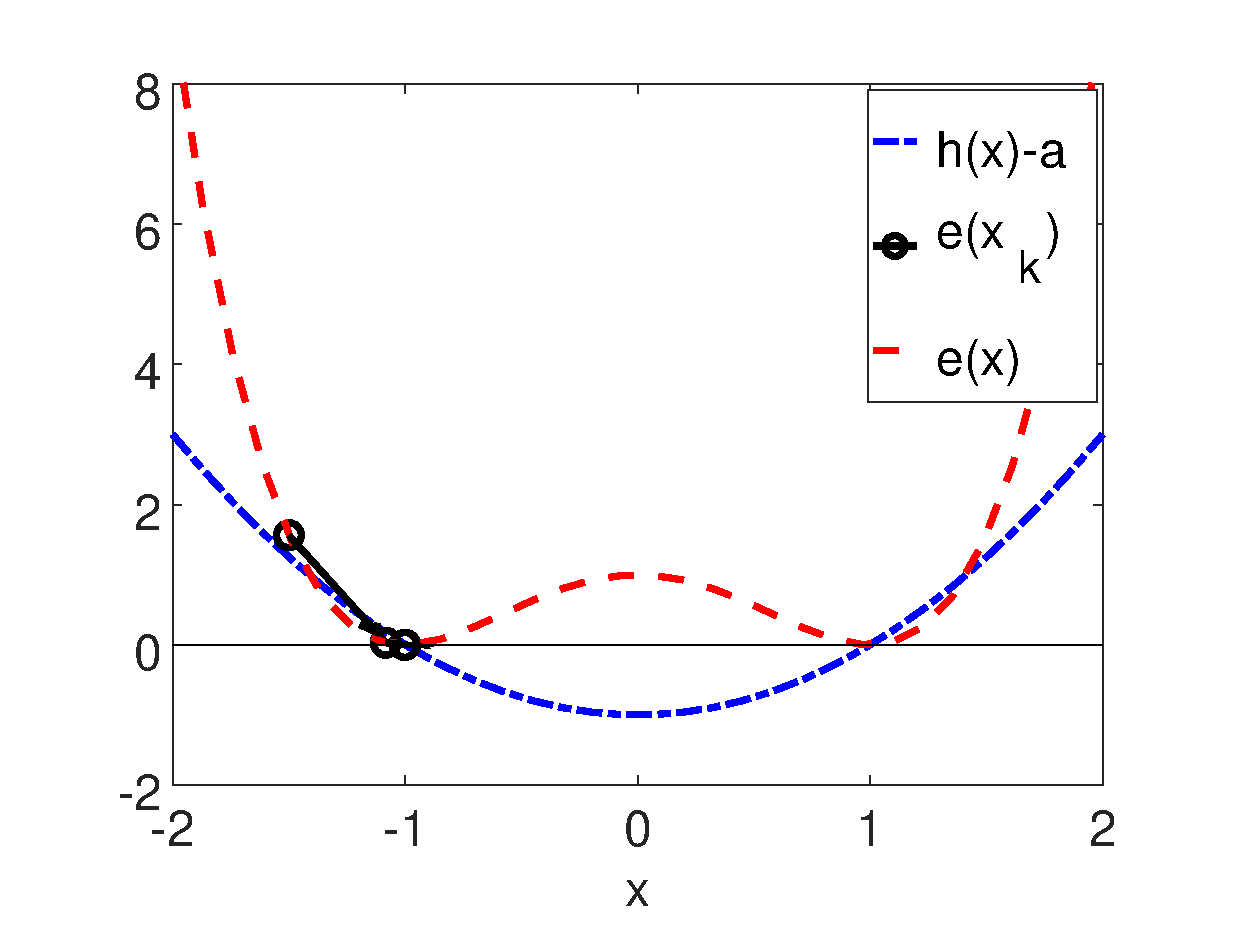
\includegraphics[width=\textwidth]{chapters/minimization-hx/mfiles/hx_a/minimizando_hx_a_1.eps}
        \caption{Usando $h(x)=x^2$ e $a=1$, quando as iterações convergem}
        \label{fig:hxacasesa}
    \end{subfigure}
    ~ %add desired spacing between images, e. g. ~, \quad, \qquad, \hfill etc. 
      %(or a blank line to force the subfigure onto a new line)
    \begin{subfigure}[b]{0.49\textwidth}
        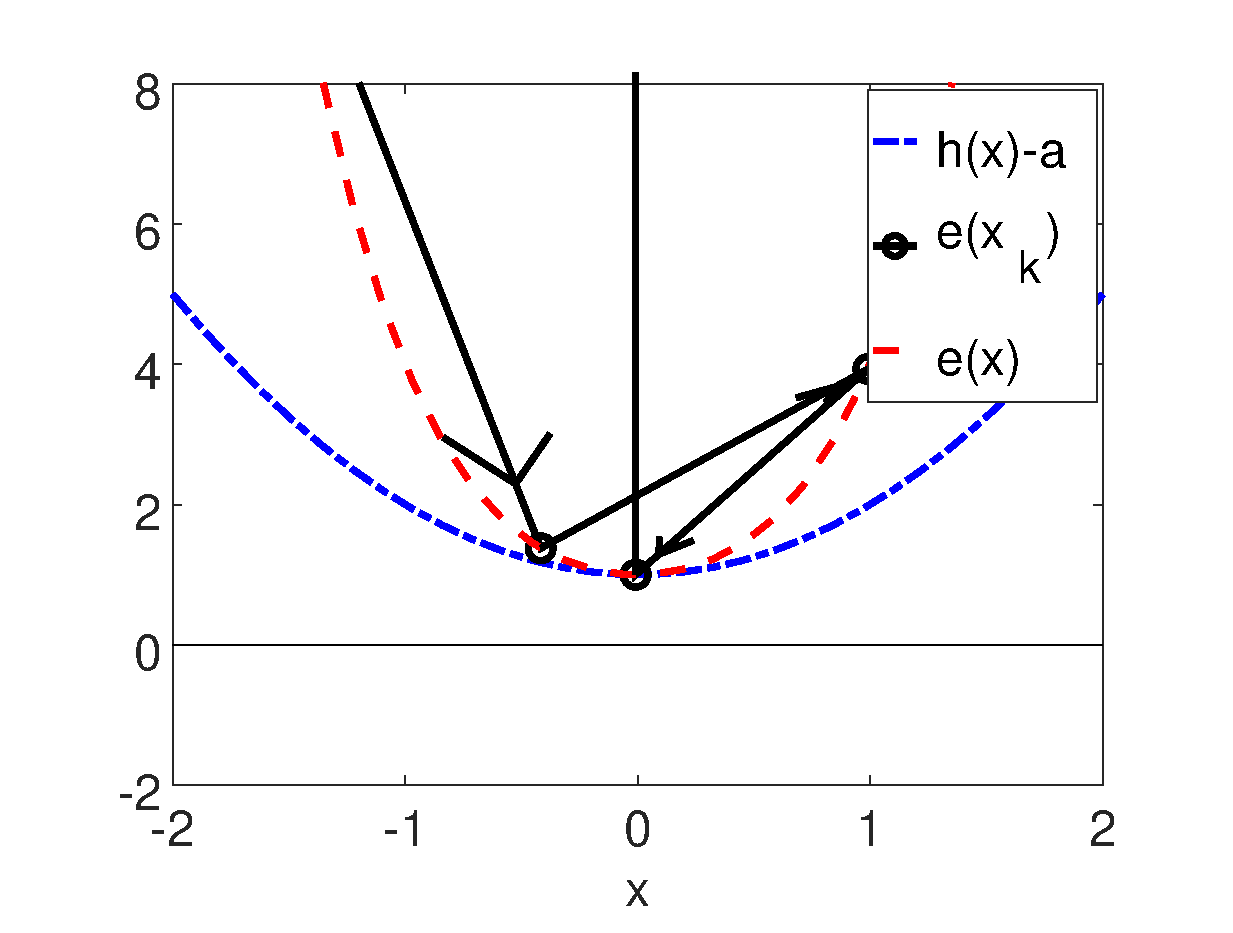
\includegraphics[width=\textwidth]{chapters/minimization-hx/mfiles/hx_a/minimizando_hx_a_2.eps}
        \caption{Usando $h(x)=x^2$ e $a=-1$, quando as iterações divergem}
        \label{fig:hxacasesb}
    \end{subfigure}
    \caption{Comportamento para $h(x)=x^2$ da equação iterativa do Teorema \ref{theo:minhxhx}}
    \label{fig:hxacases}
\end{figure}

\begin{table}[!h]
\centering
\begin{tabular}{|l|l|l|l|l|l|}
\hline
$k$      & 0 & 1 & 2 & 3 & 4 \\ \hline
$x_k$    & -1.5000 & -1.0833 & -1.0032 & -1.0000 & -1.0000 \\ \hline
$e(x_k)$ & 1.5625 & 3.0141e-02 & 4.1223e-05 & 1.0486e-10 & 6.8718e-22 \\ \hline
\end{tabular}
\caption{Resposta iterativa do Exemplo \ref{ex:minhxhx1}.}
\label{tab:hxacases1}
\end{table}

\begin{example}\label{ex:minhxhx2}
Conhecida uma função $h(x)=x^2$ é o valor $a=-1$ do contradomínio de $h(x)$,
achar o valor $x=\hat{x}$ que minimize $e(x)=(h(x)-a)^2$.
\end{example}


\begin{SolutionT}[Relativa ao Exemplo \ref{ex:minhxhx2}:]\label{sol:minhxhx2}
A Fig. \ref{fig:hxacasesb} nos mostra o processo de busca de um mínimo de $e(x)$. 
A busca inicia em $x_0=-1.5$,
 todos os valores $x_{k}$ podem ser vistos na Tabela \ref{tab:hxacases2}. 
Neste caso a busca iterativa indicada pela Eq. (\ref{eq:minhxhx2}) diverge 
em $x_3\approx 0$ com $e(x_3)=1.0001$ que é o mínimo;
ao princípio os valores de $x_{k}$ tendem a procurar o mínimo; porém,
perto de este valor se cumpre que $h'(x_{k})\cong 0$, e o valor de $x_{k}$ diverge
a um valor muito longe do mínimo; é fácil de observar, que neste caso se produz 
uma especie de efeito sanfona, onde $x_{k}$ se aproxima ao mínimo $e(x)$, e quando 
está muito próximo do mínimo o valor volta divergir.
\end{SolutionT}

\begin{table}[!h]
\centering
\begin{tabular}{|l|l|l|l|l|l|}
\hline
$k$      & 0 & 1 & 2 & 3 & 4 \\ \hline
$x_k$    & -1.5000 & -4.1667e-01 & 9.9167e-01 & -8.3683e-03 & 59.745 \\ \hline
$e(x_k)$ & 10.562 & 1.3774 & 3.9339 & 1.0001 & 1.2748e+07 \\ \hline
\end{tabular}
\caption{Resposta iterativa do Exemplo \ref{ex:minhxhx2}.}
\label{tab:hxacases2}
\end{table}

\begin{example}\label{ex:minhxhx3}
Conhecida uma função $h(x)=x^3$ é o valor $a=1$ do contradomínio de $h(x)$,
achar o valor $x=\hat{x}$ que minimize $e(x)=(h(x)-a)^2$.
\end{example}
\begin{SolutionT}[Relativa ao Exemplo \ref{ex:minhxhx3}:]\label{sol:minhxhx3}
 A Fig. \ref{fig:hxacases3a} nos mostra o processo de busca de um mínimo
 de $e(x)$, a busca inicia em $x_0=-1.5$,
 todos os valores $x_{k}$ podem ser vistos na segunda linha da
Tabela \ref{tab:hxacases3}. Neste caso a Eq. (\ref{eq:minhxhx2}) diverge em 
valores de $x_{k}$ próximos a $0$, pois provocam valores  $h'(x_{k})\approx 0$.
É fácil observar, como neste caso a busca ia na direção correta,
porém esta diverge quando $x_{k}$ se aproxima a um ponto de inflexão de $e(x)$;
nesse sentido, com mais iterações, outra direção e sorte, 
pode que seja possível atingir o mínimo de $e(x)$.
\end{SolutionT}

\begin{figure}[!h]
    \centering
    \begin{subfigure}[b]{0.49\textwidth}
        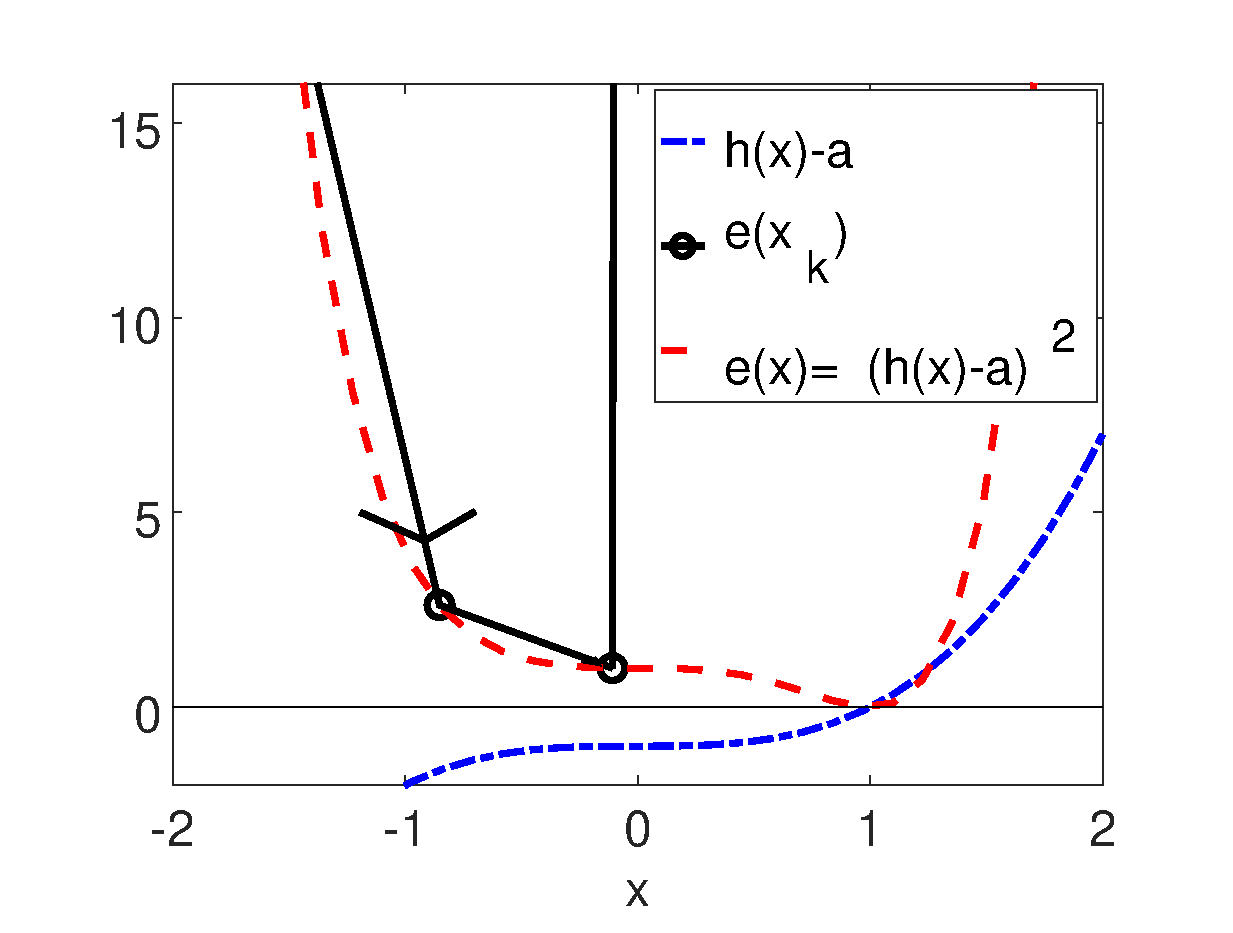
\includegraphics[width=\textwidth]{chapters/minimization-hx/mfiles/hx3_a/minimizando_hx_a_1.eps}
        \caption{Usando $h(x)=x^3$ e $a=1$, quando as iterações divergem}
        \label{fig:hxacases3a}
    \end{subfigure}
    ~ %add desired spacing between images, e. g. ~, \quad, \qquad, \hfill etc. 
      %(or a blank line to force the subfigure onto a new line)
    \begin{subfigure}[b]{0.49\textwidth}
        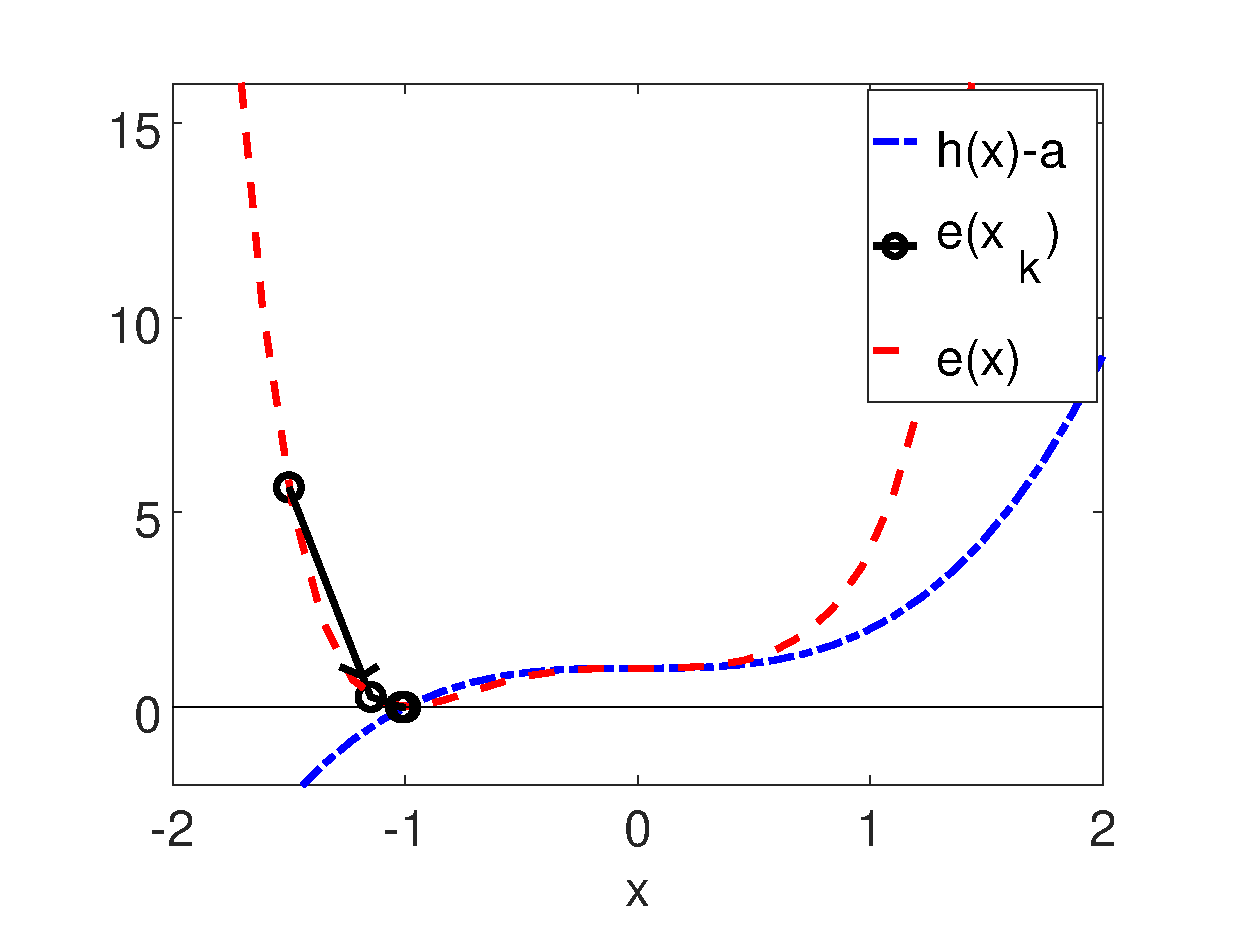
\includegraphics[width=\textwidth]{chapters/minimization-hx/mfiles/hx3_a/minimizando_hx_a_2.eps}
        \caption{Usando $h(x)=x^3$ e $a=-1$, quando as iterações convergem}
        \label{fig:hxacases3b}
    \end{subfigure}
    \caption{Comportamento para $h(x)=x^3$ da equação iterativa do Teorema \ref{theo:minhxhx}}
    \label{fig:hxacases3}
\end{figure}


\begin{table}[!h]
\centering
\begin{tabular}{|l|l|l|l|l|l|}
\hline
$k$      & 0 & 1 & 2 & 3 & 4 \\ \hline
$x_k$    & -1.50000 & -0.85185 & -0.10854 & 28.21988 & 18.81368 \\ \hline
$e(x_k)$ & 19.141 & 2.6184 & 1.0026 & 5.0500e+08 & 4.4331e+07 \\ \hline
\end{tabular}
\caption{Resposta iterativa do Exemplo \ref{ex:minhxhx3}.}
\label{tab:hxacases3}
\end{table}


\begin{example}\label{ex:minhxhx4}
Conhecida uma função $h(x)=x^3$ é valor $a=-1$ do contradomínio de $h(x)$,
achar o valor $x=\hat{x}$ que minimize $e(x)=(h(x)-a)^2$.
\end{example}
\begin{SolutionT}[Relativa ao Exemplo \ref{ex:minhxhx4}:]\label{sol:minhxhx4}
A Fig. \ref{fig:hxacases3b} nos mostra o processo de busca de um mínimo
 de $e(x)$, a busca inicia em $x_0=-1.5$,
 todos os valores de $x_{k}$ podem ser vistos na terceira coluna da
Tabela \ref{tab:hxacases4}. Neste caso a Eq. (\ref{eq:minhxhx2}) converge
em $\hat{x}\approx x_4 =-1$ com $e(\hat{x})\approx 0$, sendo este um mínimo global.
\end{SolutionT}

\begin{table}[!h]
\centering
\begin{tabular}{|l|l|l|l|l|l|}
\hline
$k$      & 0 & 1 & 2 & 3 & 4 \\ \hline
$x_k$    & -1.5000 & -1.1481 & -1.0183 & -1.0003 & -1.0000 \\ \hline
$e(x_k)$ & 5.6406e & 2.6372e-01 & 3.1238e-03 & 9.6110e-07 & 1.0241e-13 \\ \hline
\end{tabular}
\caption{Resposta iterativa do Exemplo \ref{ex:minhxhx4}.}
\label{tab:hxacases4}
\end{table}

